\section*{Dati e risultati}

\subsection*{Amplificatore operazionale open loop}

In questo paragrafo voliamo descrivere il comportamento del nostro amplificatore operazionale nella configurazione open loop. Ovvero, come illustrato in Figura \ref{fig:open_loop}, andiamo ad alimentare il nostro OPAMP con una $V\ped{cc}^+\,=\,\SI{+15}{\volt}$ e $V\ped{cc}^-\,=\,\SI{-15}{\volt}$. Colleghiamo i due ingressi, invertente ($V^-$) e non invertente ($V^+$) al comune in modo da non avere alcun segnale in ingresso al nostro amplificatore operazionale. Inoltre non inseriamo alcun circuito di retroazione. Infine colleghiamo l'output all'oscilloscopio, in modo da ottenere il valore della tensione di output ($V\ped{out}$).
A questo punto possiamo notare che: se l'amplificatore operazionale fose ideale la $V\ped{out}$ risulterebbe nulla, in quanto valgono le seguenti relazioni:

\begin{equation}
	V_d\,=\,V^+\,-\,V^- \qquad V\ped{out}\,=\,G\,V_d
\end{equation}

dove con $V_d$ si intende la differenza di potenziale tra i due ingressi dell'OPAMP e con $G$ indichiamo in guadagno del nostro amplificatore operazionale. Pertanto dal momento che i due ingressi si trovano entrambi alla stessa differenza di potenziale la loro differenza risulterebbe nulla e pertanto otterremmo $V\ped{out}\,=\,\SI{0}{\volt}$.
Al contrario per l'amplificatore operazionale reale abbiamo ottenuto che, se $V\ped{out}\,=\,\SI{0}{\volt}$, la differenza di potenziale tra i due ingressi non è 0 ma risulta essere:

\begin{equation}
	V_d\,=\,(-12.80\,\pm\,0.01) \SI{}{\volt}
\end{equation}

Questo valore ci suggerisce che il nostro amplificatore operazionale, già a valori di tensione in ingresso nulli è in saturazione negativa. Per verificare quanto appena detto abbiamo deciso di collegare $V^-$ al comune e $V^+$ a una tensione di $\SI{-15}{\volt}$, in modo che l'OPAMP, fosse sicuramente in saturazione negativa. Quello che abbiamo osservato è che il valore di $V\ped{out}$ raggiunto è di $(-12.94\,\pm\,0.01)\,\SI{}{\volt}$ che è molto vicino al valore di $V_d$ ottenuto. Quindi possiamo dire che in entrambi i casi il nostro amplificatore operazionale si trova in saturazione negativa.
La situazione sopra descritta può essere meglio compresa facendo riferimento alla Figura \ref{fig:plot_Vd}:

\begin{SCfigure}
	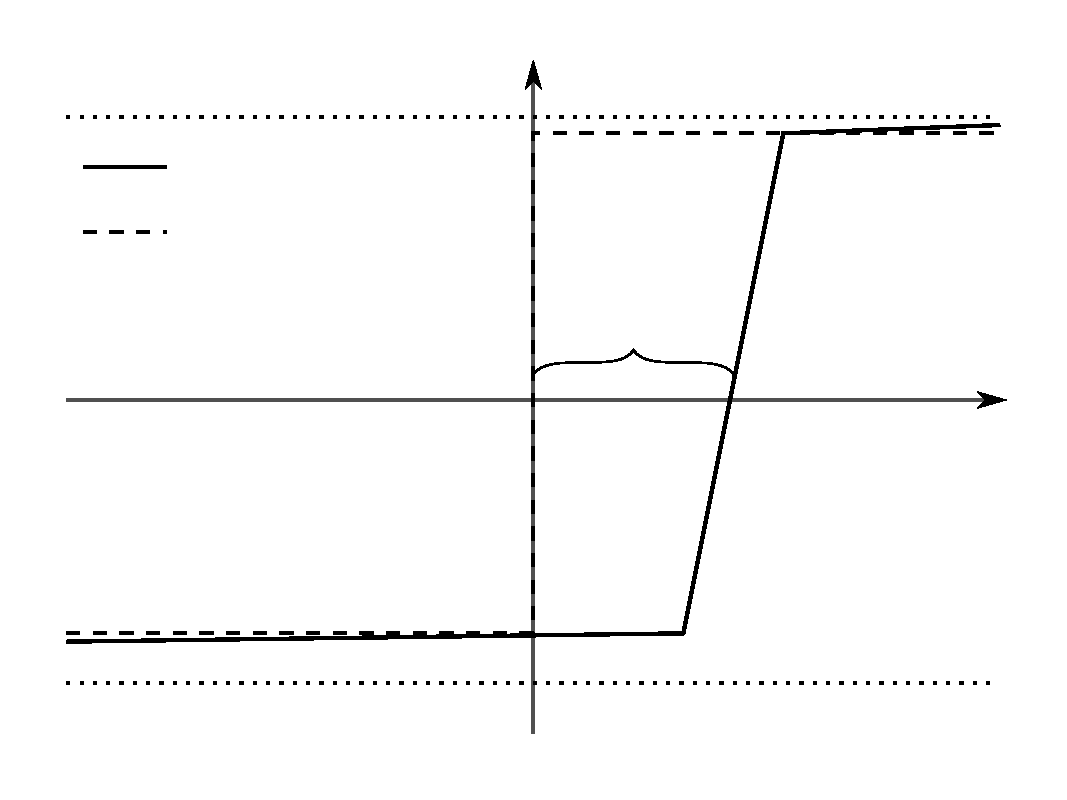
\includegraphics[width=0.45\textwidth]{../figure/offset_graph.pdf}
    \caption{Questo grafico mostra l'andamento della tensione di output $V\ped{out}$ al variare della differenza di potenziale tra i due ingressi $V_d$. Possiamo notare che se l'OPAMP fosse ben calibrato ad una $V_d=\SI{0}{\volt}$ corrisponderebbe una $V\ped{out}$ nulla, ma non è il nostro caso. Inoltre la linea tratteggiata riporta l'andamento che dovrebbe avere la $V\ped{out}$ di un amplificatore operazionale ideale, mentre la linea continua riporta l'andamento reale del nostro amplificatore operazionale UA741, dove si vede chiaramente ladifferenza di potenziale che c'è tra i due ingressi nonostante la tensione di output sia nulla.}
    \label{fig:plot_Vd}
\end{SCfigure}

\subsection*{Misura della tensione di offset}

Ricordiamo che la tensione di offset $V\ped{os}$ è quella differenza di potenziale che deve essere applicata ad un amplificatore operazionale per ottenere in uscita una tensione nulla.

A livello teorico, l'output di un amplificatore operazionale dovrebbe assumere un valore di potenziale nullo quando ad entrambi i suoi ingressi viene applicata la stessa differenza di potenziale. In realtà, negli OPAMP reali ciò non accade. Per questo motivo gli amplificatori operazionali presentano una coppia di pin il cui impiego è quello di permettere la taratura della tensione di offset tramite un trimmer. La differenza tra le correnti dei due ingressi quando l'amplificatore operazionale è a riposo è detta corrente di offset.

Quindi al fine di misurare la tensione di offset del nostro amplificatore operazionale abbiamo montato il circuito riportato in Figura \ref{fig:offset} e lo abbiamo dimensionato in modo da determinare i valori più intelligenti di resistenza atti ad ottenere una buona stima di $V\ped{os}$.
Come per il circuito precedente abbiamo che $V\ped{cc}^+\,=\,\SI{+15}{\volt}$ e $V\ped{cc}^-\,=\,\SI{-15}{\volt}$.
In questo caso, sfruttando le regole per gli OPAMP e un po' di analisi circuitale, abbiamo ottenuto che:

\begin{equation}
	\left\{
  \begin{array}{l l l}
    I_1\,=\,\frac{V_a\,-\,0}{R_1}\\
    I_2\,=\,\frac{V\ped{out}\,-\,V_a}{R_2}\\
    I_1\,=\,I_2\,+\,I_{p}^-
  \end{array} \right.\
  \label{eq:sistema}
\end{equation}

\begin{equation}
	V\ped{out}\,=\,I_2R_2\,+\,V_a
	\label{eq:offset}
\end{equation}

dove, facendo riferimento alla Figura \ref{fig:offset}, abbiamo che $I_1$ è la corrente che passa per $R_1$, $I_2$ è la corrente del ramo di retroazione negativo, $I_{p}^-$ è la corrente di polarizzazione negativa, $V_a$ è la tensione presente sul nodo dell'ingresso invertente.
Quindi con una serie di banali passaggi matemtici che sfruttano le relazioni \ref{eq:offset} e \ref{eq:sistema} e osservando che, in questa configurazione, $V\ped{os}\,\equiv\,V_a$ otteniamo il seguente risultato:

\begin{equation}
	V\ped{out}\,=\,V\ped{os}\left(1+\frac{R_2}{R_1}\right)\,-\,I_{p}^-R_2
	\label{eq:offset1}
\end{equation}

Quindi, ricordandoci che le correnti di polarizzazione sono dell'ordine di qualche decina di $\SI{}{\nano\ampere}$, abbiamo scelto i valori delle resistenze $R_1$ e $R_2$ in modo da minimizzare il contributo di $I_{p}^-R_2$. Pertanto abbiamo scelto i seguenti valori di resistenza: $R_1\,=\,\SI{10}{\ohm}$ e $R_2\,=\,\SI{10}{\kilo\ohm}$.
Infine abbiamo ricavato il valore di $V_a$ invertendo la relazione \ref{eq:offset1} nella quale abbiamo trascurato l'effetto del termine $I_{p}^-R_2$, ottenendo:

\begin{equation}
	V\ped{os}\,\simeq\,V\ped{out}\frac{R_1+R_2}{R_1}\,=\, (0.97 \pm 0.07)\SI{}{\milli\volt}
\end{equation}

Infine abbiamo anche preso una misura diretta della tensione di offset che è risultata essere: $V\ped{os}\,=\,(1.09\pm0.01)\SI{}{\milli\volt}$. Si può osservare che i due valori sono quasi compatibili entro le loro incertezze, quindi con spirito ottimistico possiamo affermare che in entambi i casi abbiamo raggiunto dei valori plausibili.

\subsection*{Azzeramento di $V\ped{os}$ grazie al Trimmer}

In questo paragrafo ci poniamo il problema di azzerare il valore della tensione di offset $V\ped{os}$. Per farlo abbiamo realizzato il circuito riportato in Figura \ref{fig:trimmer}.
Per questo circuito, come per quelli precedenti le tensioni di alimentazione sono $V\ped{cc}^+\,=\,\SI{+15}{\volt}$ e $V\ped{cc}^-\,=\,\SI{-15}{\volt}$.
Possiamo notare che in questa configurazione il terminale non invertente è collegato al comune, mentre quello invertente è collegato direttamente al ramo di retroazione negativo, e quindi abbiamo un emitter follower.
Quindi, al fine di avere una tensione di offset nulla, abbiamo variato manualmente il valore della resistenza variabile $R_v$ fino a che non abbiamo ottenuto un valore nullo della tensione di output, $V\ped{out}\,=\,\SI{0}{\volt}$.
In questo modo abbiamo effettiavamente ottenuto un OPAMP per cui, collegando al comune i due ingressi, la differenza di potenziale di output risulta effettivamente nulla, come per un amplificatore operazionale ideale.

Quindi ricordando che $R_v$ ha un range di valori possibili compreso tra $0$ e $10$ $\SI{}{\kilo\ohm}$ riportiamo i valori delle due resistenze $R\ped{1-4}$ e $R\ped{4-5}$ che indicano rispettivamente il valore di resistenza tra il pin 1 e 4  e tra il 4 e il 5 dell'amplificatore operazionale. I valori ottenuti sono:

\begin{equation}
	R\ped{1-4}\,=\,(6.158\,\pm\,0.001)\SI{}{\kilo\ohm} \qquad \textbf{e} \qquad R\ped{4-5}\,=\,(4.417\,\pm\,0.001)\SI{}{\kilo\ohm}
\end{equation}

Salta subito all'occhio che la somma dei due valori di resistenze, che sono in serie, è maggiore di $\SI{10}{\kilo\ohm}$. Questo non è errato dal momento che il valore messimo di $R_v$ e superiore a $\SI{10}{\kilo\ohm}$, in quanto lo abbiamo misurato col multimetro.

\subsection*{Studio delle correnti di polarizzazione}

Perchè un amplificatore operazionale reale presenta delle correnti che scorrono nei suoi ingressi nonostante il valore elevato della resistenza di ingresso? Questo avviene perchè lo stadio di ingresso è costituito da un amplificatore differenziale che, per funzionare correttamente, deve avere i transistor opportunamente polarizzati. Questo comporta l'esistenza di correnti continue di polarizzazione che sono appunto $I_{p}^-$ e $I_{p}^+$.

Pertanto ora che siamo riusciti a trovare il valore della tensione di offset ($V\ped{os}$) e ad eliminarla quasi del tutto grazie all'impiego di un trimer, possiamo concentrarci nella ricerca di un modo per misurare le correnti di polarizzazione dei due ingressi ($I_{p}^-$ per l'ingresso invertente e $I_{p}^+$ per l'ingresso non invertente).

Dal momento che le due correnti hanno un'intensità molto piccola, dell'ordine di $\SI{}{\nano\ampere}$ non possiamo misurarle direttamente. Per questo motivo abbiamo deciso di sfruttare la legge di Ohm che lega la differenza di potenziale ai capi di una resistenza ala corrente che vi scorre secondo la legge: $\Delta V\,=\,IR$. A tal fine abbiamo scelto un valore di resistenza $R_3$ elevato (dell'ordine di $\SI{}{\kilo\ohm}$) in modo che la differenza di potenziale potesse essere misurata agevolmente. Quindi abbiamo realizzato i seguenti circuiti:

\begin{figure}[H]
        \centering
        \begin{subfigure}[b]{0.45\textwidth}
                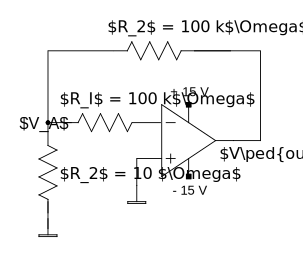
\includegraphics[width=\textwidth]{../figure/Ip_minus.pdf}
                \caption{Amplificatore operazionale: configurazione per la misura di $I_{p}^-$}
                \label{fig:ip_minus}
        \end{subfigure}
        ~
        \begin{subfigure}[b]{0.45\textwidth}
                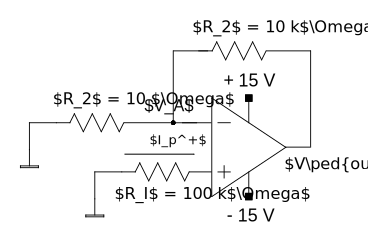
\includegraphics[width=\textwidth]{../figure/Ip_plus.pdf}
                \caption{Amplificatore operazionale: configurazione per la misura di $I_{p}^+$}
                \label{fig:ip_plus}
        \end{subfigure}
        \caption{Questi circuiti illustrano le configurazioni adottate per misurare le due correnti di polarizzazione riferite ai due ingressi (invertente e non invertente) dell'amplificatore operazionale.}
        \label{fig:circuits}
\end{figure}

La procedura che abbiamo seguito per ricavare i valori delle due correnti è stata relativamente semplice.
\begin{itemize}\itemsep2pt \parskip0pt \parsep0pt
	\item{Con lo stesso procedimento illustrato nel paragrafo precedente abbiamo annullato la tensione di offset del nostro amplificatore operazionale;}
	\item{Successivamente abbiamo sistemato le resistenze nei nostri circuiti. Le resistenze hanno i seguenti valori: $R_1=\SI{10}{\ohm}$, $R_2=\SI{10}{\kilo\ohm}$ e $R_3=\SI{100}{\kilo\ohm}$ per entrambe le configurazioni. Figura \ref{fig:ip_minus} e \ref{fig:ip_plus};}
	\item{Quindi siamo andati a calcolare il valore delle due intensità di corrente di polarizzazione sia sfruttando la legge di Ohm, e quindi con una misura diretta della diferenza di potenziale ai capi della resistenza $R_3$, sia risolvendo il circuito e misurando la tensione di offset, quest'ultima solo per l'ingresso invertente;}
\end{itemize}

\subsubsection*{Misura della corrente di polarizzazione $I_{p}^-$}

Il valore della corrente di polarizzazione ottenuto grazie alla misura diretta della tensione ai capi della resistenza (Figura \ref{fig:ip_minus}) è il sguente:

\begin{equation}
	I\ped{p1}^-\,=\,\frac{\Delta V}{R_3}\,=\,(\,\pm\,)\,\SI{}{\nano\ampere}
\end{equation}

Mentre, se vogliamo calcolare $I_{p}^-$ sfruttando il valore della tensione di output, quindi risolvendo il circuito, dobbiamo, come prima cosa, ricavare l'equazione che lega $V\ped{out}$ con i vari parametri circuitali: resistenze e tensioni del circuito. Questa equazione, già ottenuta nel secondo paragrafo di queso elaborato, è:

\begin{equation}
	V\ped{out}\,=\,V_a\left(1+\frac{R_2}{R_1}\right)\,-\,I_{p}^-R_2 \qquad \text{con} \qquad V_a\,=\,I_{p}^-R_3
\end{equation}

quindi con una serie di passaggi algebrici possiamo ottenere la seguente espressione:

\begin{equation}
	V\ped{out}\,=\,I_{p}^-\,\left(R_3+\frac{R_2}{R_1}R_3-R_2\right)
\end{equation}

dalla quale otteniamo che il valore della corrente di polarizzazione dell'ingresso invertente ha valore:

\begin{equation}
	I\ped{p2}^-\,=\,(\,\pm\,)\,\SI{}{\nano\ampere}
\end{equation}

e come si può osservare le due misure $I\ped{p1}^-$ e $I\ped{p2}^-$ risultano essere compatibili entro le loro incertezze.

\subsubsection*{Misura della corrente di polarizzazione $I_{p}^+$}

Il valore della corrente di polarizzazione ottenuto grazie alla misura diretta della tensione ai capi della resistenza è il sguente:

\begin{equation}
	I\ped{p}^+\,=\,\frac{\Delta V}{R_3}\,=\,(30\,\pm\,10)\,\SI{}{\nano\ampere}
\end{equation}

In questo caso non abbiamo avuto voglia di risolvere il circuito e quindi di verificare che il valore trovato di $I\ped{p}^+$ risulti compatibile con quello che avremmo potuto ottenere risolvendo il circuito nella configurazione illustrata in Figura \ref{fig:ip_plus}.